A hipótese base desse trabalho é que, baseado nos projetos mencionados anteriormente,
é possível implementar um novo modelo de gerador que seja muito mais extensível, amigável
e que consiga implementar funcionalidades mais genéricas. Além disso, outra hipótese
é que, com base nessa extensibilidade, conseguimos aumentar de forma considerável a
eficiência de um time de desenvolvimento, utilizando o gerador para automatizar
trabalhos repetitivos.

\section{\Baker{}}

O projeto desenvolvido nesse trabalho, e seu resultado principal, é o programa \Baker{}
\cite{baker}, uma plataforma para desenvolvimento de geradores de código componentizáveis.
O projeto usa como base a IDL Protocol Buffers, por ser mais amigável ao desenvolvedor e
por possuir um ecossitema maduro de ferramentas de análise e de suporte.

Com foco em extensibilidade, o projeto tenta realizar o minímo de escolhas que impeçam ou
dificultem autores de construir geradores na plataforma. Além disso, as interfaces entre o
programa e os geradores foram pensadas para facilitar a construção programática e estruturada
do código, ao invés de ser baseada em texto ou processador de \textit{templates}.

O programa separa geradores em dois tipos, cada um responsável por parte do fluxo de geração:

\begin{itemize}
\item \textit{Layers}: Programas responsáveis por gerar, a partir das estruturas construidas
  a partir dos arquivos fonte do usuário, fragmentso de código na linguagem intermediária (IR)
  do projeto. Cada \textit{layer} é responsável por gerar apenas parte do resultado final, os
  resultados de cada uma são combinados para formarem a estrutura intermediária final.
\item \textit{Codegens}: Programa responsável por, a partir da estrutura em IR gerada por todas
  as \textit{layers}, gerar o código final na linguagem objeto.
\end{itemize}

A escolha em separar os geradores nessas duas categórias é devida aos seguintes fatores:

\begin{itemize}
\item Ao limitarmos a lógica de tradução IR $\rightarrow$ linguagem objeto aos \textit{codegens},
  e que esses possuam apenas essa lógica, permitimos que \textit{layers} se preocupem apenas com
  \textit{qual} código deve ser gerado, e não em \textit{como}.
\item Pelo mesmo motivo, diminuimos o custo de construção de novas \textit{layers}, já que o
  trabalho que essas precisam realizar é menor. Além disso, simplificamos a troca de uma \textit{layer}
  por outra que gere uma integração com a mesma biblioteca de uma forma diferente, aumentando o
  grau de customização pelos usuários.
\item O fato de combinarmos os resultados de todas as \textit{layers} de forma estruturada e clara
  permite que cada uma seja responsável por apenas parte do código final, sem depender que códigos
  anteriores tenham gerados os \textit{entrypoints} necessários (quando comparado com
  \textit{plugins} de \cite{googl:protobuf}).
\item O foco na construção programática do código diminui a barreira de entrada para novos
  desenvolvedores, já que técnicas padrão de desenvolvimento de software podem ser aplicadas sem
  dificuldades, pois todos os dados que o desenvolvedor lida são estruturados.
\end{itemize}

\subsection{Representação Intermediária (IR)}

A IR utilizada pelo programa para armazenar o código a ser gerado é, na realidade, apenas um
conjunto de estruturas definidas em Protocol Buffers, não possuindo representação textual e
muitas dessas estruturas não possuem comportamento definidos. Essas estruturas possuem apenas
o mínimo de especificação para que autores de \textit{layers} e \textit{codegens} sejam capazes
de mapear cada estrutura para um análogo na linguagem objeto. Essa escolha é feita para evitar
que \Baker{} limite o que pode ser gerado.

Como veremos, o fato da IR ser definida em Protocol Buffers possibilita que geradores sejam
construidos em qualquer linguagem que possua suporte ao formato.

A IR é estruturada da seguinte maneira:

\begin{itemize}
\item Cada arquivo fonte é ligado a uma (ou mais) \texttt{IrFile}s.
\item Cada \texttt{IrFile} contém um \texttt{Namespace} raiz.
\item \texttt{Namespace}s são responsáveis por armazenar definições a serem geradas, esses podem ser:
  funções, tipos (que podem ser \textit{record types}, e.g. \texttt{struct}s, ou \textit{sum types},
  e.g. \texttt{enum}s), funções, interfaces, constantes ou mesmo outros \texttt{Namespace}s. Podemos
  pensar em um \texttt{Namespace} dentro de outro como uma forma de expressar submódulos, mas também
  pode ser usado para declarar estruturas dentro de outras (e.g. uma classe dentro de outra).
\item Declarações de tipos contém tanto a estrutura do tipo em si (propriedades ou membros), como
  também atributos aplicados ao tipo, documentação e uma série de \texttt{ImplBlock}s.
\item \texttt{ImplBlock} é usado para definir uma série de implementações para um tipo específico,
  como implementar uma certa interface, adicionar métodos, etc. Em cada bloco, uma série de restrições
  podem ser adicionadas, e.g. limitar genéricos a implementarem uma dada interface. A separação em
  uma série de blocos simplifica a implementação de \textit{layers} e também leva em conta que
  existem linguagens com essa funcionalidade.
\end{itemize}


\subsection{Processo de Geração}

Com essas definições em mãos, o fluxo do programa é:

\begin{enumerate}
\item A partir dos arquivos fonte passados, processamos pacotes, mensagens, serviços e enums
  definidos nos mesmos. Esse processo requer identificar corretamente, a partir do escopo atual,
  a qual estrutura cada campo se refere. No final desse processo, o grafo contém a lista
  normalizada das estruturas declaradas. Uma lista não exaustiva do processo de normalização é:

  \begin{itemize}
  \item Todos os nomes das estruturas são convertidos para nomes absolutos (pacote + escopo + nome),
    e.g. \texttt{Foo} é convertido para \texttt{foo.v1.Foo};
  \item Linhas de documentação são combinadas em um único texto;
  \item Referências a nomes de estruturas são convertidos para os identificadores das mesmas no
    grafo. Permitindo que sejam facilmente buscadas.
  \item Convertemos diversas estruturas padrões de Protocol Buffers para tipo normalizados, que
    podem ser usados mais facilmente por \textit{layers}, e.g. o tipo \texttt{google.protobuf.Timestamp}
    é convertido para o tipo normalizado \texttt{TIMESTAMP}.
  \end{itemize}

  Esse processo é realizado pela entidade denominada \textit{Proto Loader}.
\item Enviamos o grafo gerado para cada uma das \textit{layers}, em ordem recebida pelo programa.
  Cada uma dessas responde com um pedaço de código na IR do projeto.
\item Todas as respostas em IR são combinadas em uma única estrutura. O processo de combinação é
  uma possível área de melhoria, sendo feito, no momento de escrita, as seguintes combinações:

  \begin{itemize}
  \item Para cada \textit{namespace}, combinamos todos as definições entre duas respostas.
  \item Para definições de tipos com o mesmo nome, caso ambas as definições sejam do mesmo formato:
    \begin{enumerate}
    \item No caso de \textit{record types}, combinamos todas as propriedades em ambas as definições.
      Caso a mesma propriedade exista em ambas, a visibilidade é modificada para a mais permissiva e
      atributos são agrupados.
    \item No caso de \textit{sum types}, agrupamos apenas atributos em membros que existam em ambas
      as definições. É possibilidade de se adicionar novos membros a um \textit{sum type} é uma questão
      em aberto, devido a facilidade de gerar códigos objeto invalidos.
    \end{enumerate}
  \item Outras definições são apenas agrupadas.
  \end{itemize}

  Esse processo é realizado pela entidade denominada \textit{IR Merger}.
\item A estrutura final é enviada para o \textit{codegen} final, que fará a conversão para código
  objeto e também \textit{salvará o arquivo final em disco}. O fato do \textit{codegen} fazer a
  escrita em disco é para darmos flexibilidade e permitimos outros tipos de geração, e.g. usar
  a IR para realizarmos migrações em bancos de dados.
\end{enumerate}

A \cref{fig:baker-data-flow} apresenta um digrama simplificado do fluxo de dados do programa.

\begin{figure}[h]
  \centering
  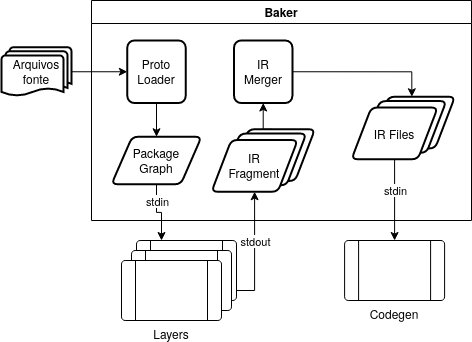
\includegraphics[width=0.8\linewidth]{Imagens/baker-diagram.png}
  \caption{Digrama do Fluxo de Dados do programa}
  \label{fig:baker-data-flow}
\end{figure}

\subsection{Comunicação Entre Programas}

Para permitir que os programas sejam escritos no maior número de linguagens de programação, a comunicação
entre o programa principal, \textit{layers} e \textit{layers} é feita de forma similar a plugins para
\cite{googl:protobuf}: toda a comunicação é feita via entrada e saída padrão e utilizando Protocol Buffers
como formato. A saida padrão para erros é redirecionada para a saida padrão do programa como um todo, para
facilitar o relato de erros ao usuário.

O uso de Protocol Buffers ao invés de um formato customizado ou até mesmo JSON é devido a:

\begin{itemize}
\item Por ser a IDL utilizada, mantemos o padrão e simplificamos o fluxo.
\item Garante que as estruturas sejam construidas e geradas corretamente.
\item Facilita a manutenção de compatibilidade com \textit{layers} baseadas em versões anteriores
  da ferramenta.
\end{itemize}
